\documentclass{ximera}

%\newtheorem{theorem}{Theorem}%[section] % reset theorem numbering for each section
%\newtheorem*{theorem*}{Theorem}%[section] % reset theorem numbering for each section
%\newtheorem{prop}[theorem]{Proposition}
%\newtheorem{lem}[theorem]{Lemma}
%\newtheorem{ex}{Example}


\title{April 22--$n$-ary expansions and Gaussian integers}  
\begin{document}  
\begin{abstract}  We look at binary and other expansions of real numbers. We also return to Gaussian integers.
\end{abstract}  
\maketitle  

\begin{definition} Let $n\in\mathbb{Z}$ with $n\geq 2$. Then every real number $\alpha\in\mathbb{R}$ with $0\leq\alpha<1$. can be uniquely written as 
\[\displaystyle\sum_{k=1}^\infty \frac{a_k}{n^k}=0.a_1a_2a_3\dots,a_k=a_k(x)\in\{0,1,\dots,n-1\}.\] We call this the $n$-ary expansion of $\alpha$. When $n=2,$ we call this binary, when $n=10,$ we call this decimal, and when $n=16,$ we call this hexidecimal.

We can expand this definition to all real numbers $x$, but the sum notation is more awkward. Typically we write something like
 \begin{align*}
 \displaystyle\sum_{k=-\infty}^\infty {b_k}{n^k}&=\dots b_2b_1b_0.b_{-1}b_{-2}b_{-3}\dots\\
 &=\cdots+b_2 n^2+b_1 n+b_0+\frac{b_{-1}}{n}+\frac{b_{-2}}{n^2}+\cdots, 
& b_k=b_k(x)\in\{0,1,\dots,n-1\},\end{align*} 
 except there will be some $K\in\mathbb{Z}$ where $b_k=0$ for all $k\geq K$. The $b_k$ (or $a_k$ in the first definition) are called \emph{digits}.
\end{definition}

\begin{example}
 When we look at the decimal expansion of a number $x$, we ask how many $10^{i}$ add up to $x$. If $x=2314.123$, there are two $10^3$, three $10^2$, one $10^1$, four $10^0$, one $10^{-1}$, two $10^{-2}$, and three $10^{-3}$ (this may give you elementary school flash backs). We use this information to fill out the chart:
 
\begin{tabular}{|c|c|c|c|c|c|c|}\hline
 $10^3$& $10^2$& $10^1$& $10^0$&$10^{-1}$&$10^{-2}$&$10^{-3}$\\\hline
 $\answer{2}$&$\answer{3}$&$\answer{1}$&$\answer{4}$&$\answer{1}$&$\answer{2}$&$\answer{3}$\\\hline
 \end{tabular}

Now, to calculate binary, we do a similar thing, but count how many $2^n$ are in a number. We started with something easier: $x$ with decimal expansion $43.75$. Remember all binary digits are $0$ or $1$

\begin{tabular}{|c|c|c|c|c|c|c|c|c|c|}\hline
 $2^5=32$& $2^4=16$& $2^3=8$& $2^2=4$& $2^1=2$& $2^0=1$&$2^{-1}=\frac{1}{2}$&$2^{-2}=\frac{1}{4}$&$2^{-3}=\frac{1}{8}$\\\hline
 $\answer{1}$&$\answer{0}$&$\answer{1}$&$\answer{0}$&$\answer{1}$&$\answer{1}$&$\answer{1}$&$\answer{1}$&$\answer{0}$\\\hline
 \end{tabular}
 
 Finally, we do a hexidecimal for $x$ with decimal expansion $2314.125$. Normally hexidecimal has $a=10, b=11,c=12,d=13,e=14,d=15$, since we need more than 10 characters, but the for the table, we will just use $10,11,12,13,14,15$.
 
 \begin{tabular}{|c|c|c|c|c|}\hline
$16^2=256$& $16^1=16$& $16^0=1$&$16^{-1}=\frac{1}{16}$&$16^{-2}=\frac{1}{256}$\\\hline
 $\answer{9}$&$\answer{0}$&$\answer{10}$&$\answer{2}$&$\answer{0}$\\\hline
 \end{tabular}
\end{example}
\begin{definition}
If there exist a positive integer $\rho$ and $N$ such that $a_k=a_{k+\rho}$ for all $k\geq N$, then the $n$-ary expansion of $\alpha$ is \emph{eventually periodic}; the sequence $a_Na_{N+1}\cdots a_{N+\rho-1}$ with $\rho$ minimal is the \emph{period} of $\alpha$ and $\rho$ is the \emph{period length}. If the smallest such $N$ is $1$, then $\alpha$ is \emph{periodic.}  An eventually periodic real number
 \[\alpha=0.a_1a_2a_3\dots a_{N-1}a_Na_{N+1}\cdots a_{N+\rho-1}a_Na_{N+1}\cdots a_{N+\rho-1}a_Na_{N+1}\cdots a_{N+\rho-1}\cdots\] is written \[\alpha=0.a_1a_2a_3\dots a_{N-1}\overline{a_Na_{N+1}\cdots a_{N+\rho-1}}.\]
\end{definition}

\begin{theorem}
 Let $\alpha\in\mathbb{R}$ with $0\leq\alpha<1$. If $\alpha$ had an finite or eventually periodic $n$-ary expansion for $n\geq 2$, then $\alpha\in\mathbb{Q}$.
\end{theorem}

\begin{theorem}
 Let $n\in\mathbb{Z}, n\geq 2$ and $x\in[0,1)$. Then
 
\begin{enumerate}
 \item $x$ has a finite $n$-ary expansion if and only if there exist $p,q\in\mathbb{Z}^{+},(p,q)=1,x=\frac{p}{q},$ and $p_i\mid n$ for all $p_i\mid q$ for $p_i$ prime.
 \item $x$ has a purely-periodic $n$-ary expansion if and only if there exist $p,q\in\mathbb{Z}(p,q)=1,x=\frac{p}{q},$ and $(q,n)=1$.
\end{enumerate}
\end{theorem}


For $n\in\mathbb{Z},n\geq2$, divide the unit interval $[0,1)$ into intervals $\left[\frac{i}{n},\frac{i+1}{n}\right)$ where $i=0,1,2,\dots,n-1$. If a number $x\in\left[\frac{i}{n},\frac{i+1}{n}\right)$, then the first digit of the $n$-art expansion is $i$

For example, binary divides partitions $[0,1)$ into $[\answer{0},\answer{\frac{1}{2}})$ and $[\answer{\frac{1}{2}},\answer{1})$. $5$-ary partitions $[0,1)$ into $[\answer{0},\answer{\frac{1}{5}})$,$[\answer{\frac{1}{5}},\answer{\frac{2}{5}})$, $[\answer{\frac{2}{5}},\answer{\frac{3}{5}})$,$[\answer{\frac{3}{5}},\answer{\frac{4}{5}})$, and 
$[\answer{\frac{4}{5}},\answer{1}).$ 

To get the second digit, we break each of these intervals into $n$ smaller intervals $\left[\frac{i}{n}+\frac{j}{n^2},\frac{i}{n}+\frac{j+1}{n^2}\right), 0\leq i\leq n-1,0\leq j\leq n-1$. For each $x\in\left[\frac{i}{n}+\frac{j}{n^2},\frac{i}{n}+\frac{j+1}{n^2}\right), x=0.ij\dots.$ 
For example, the partition for the $(1/4)^{th}$ digit in binary is $[\answer{0},\answer{\frac{1}{4}})$, $[\answer{\frac{1}{4}},\answer{\frac{2}{4}})$, $[\answer{\frac{1}{2}},\answer{\frac{3}{4}})$, and $[\answer{\frac{3}{4}},\answer{1})$.

Determining the rest of the digits involves iterating this process.

\section*{Back to Gaussian Integers and Divisibilty}
Instead of looking at other ways of writing real numbers, we can look at imaginary numbers.
Remembering back to the January, the \emph{Gaussian integers $\mathbb{Z}[i]$} are the set of complex numbers $\{a+bi:a,b\in\mathbb{Z}, i^2=-1\}$. We define addition and subtraction as normal: \[a+bi+c+di=(a+c)+(b+d)i,\quad (a+bi)(c+di)=(ac-bd)+(ad+bc)i.\]

$ab=1$ has four solutions: $a=b=\pm1$ and $a=-b=\pm i$. In this new setting, it is not clear what it means for $1<a+bi$. Is $1<-1+2i$?

\begin{definition}
 A number $p\in\mathbb{Z}[i]$ is \emph{prime} if $p\mid ab$ implies $p\mid a$ or $p\mid b$ for all $a,b\in\mathbb{Z}[i]$.
\end{definition}

Now, a quick note about the regular integers: $2=(1+i)(1-i)$, so is not prime in $\mathbb{Z}[i]$. Our goal is to show which integers are prime in $\mathbb{Z}[i]$.

\begin{theorem}
 The primes in $\mathbb{Z}[i]$ have the form:
\begin{itemize}
 \item  $p\in\mathbb{Z}$ where $p$ is a prime and $p\equiv 3 \pmod 4$
 \item $a+bi$ where $a^2+b^2$ is prime.
\end{itemize}
\end{theorem}

\begin{theorem}[Contrapositive of Textbook Lemma 2.14]
 $a^2+b^2\not\equiv 3 \pmod 4$.
\end{theorem}

\begin{theorem}[Textbook Lemma 2.13]
 If $p$ is prime and $p\equiv 1 \pmod 4$, then there exist $a,b\in\mathbb{Z}$ such that $a^2+b^2=p$.
\end{theorem}
We can use this to see that $p=(a+bi)(a-bi)$. So our only candidates for primes $a+0i$ are those congruent to 3 mod 4.

\begin{definition}
 A \emph{unit} is a Gaussian (or regular) integer $u$ where $u\mid 1$. The units in $\mathbb{Z}$ are $1,-1$, and the units in $\mathbb{Z}[i]$ are $1,-1,i,-i$.
\end{definition}

\begin{definition}
 The \emph{Gaussian norm} is $N(a+bi)=a^2+b^2$. The norm is completely multiplicative, since $N((a+bi)(c+di))=(ac-bd)^2+(ad+bc)^2=(a^2+b^2)(c^2+d^2)$.
\end{definition}

How would we divide $237+504i$ by $15-17i$? Well, we could require that the remainder is less that $N(15-17i)=514$. In this case,
\[237+504i=(-10+23i)(15-17i)+(-4-11i),\] and $N(-4-11i)=137<N(15-17i)=514$.

\begin{theorem}[Division algorithm for Gaussian integers]
 Let $\alpha,\beta\in\mathbb{Z}[i]$ with $\beta\neq 0$. Then there are Gaussian integers $\gamma$ and $\rho$ so that 
 \[\alpha=\beta\gamma+\rho\quad N(\rho)<N(\beta).\]
\end{theorem}
\begin{proof}
 If with divide the equation we are trying to solve by $\beta$, it becomes \[\frac{\alpha}{\beta}=\gamma+\frac{\rho}{\beta}\quad N(\frac{\rho}{\beta})<1.\]
 If the ratio $\frac{\alpha}{\beta}$ is a Gaussian integer, then $\gamma=\frac{\alpha}{\beta}$ and $\rho=0$. Otherwise, $\frac{\alpha}{\beta}$ is in a square with corners $a+bi, a+1+bi, a+(b+1)i,a+1+(b+1)i.$ We set $\gamma$ equal to the closest corner of the square to $\frac{\alpha}{\beta}$ as in the image.
 
\begin{image}
  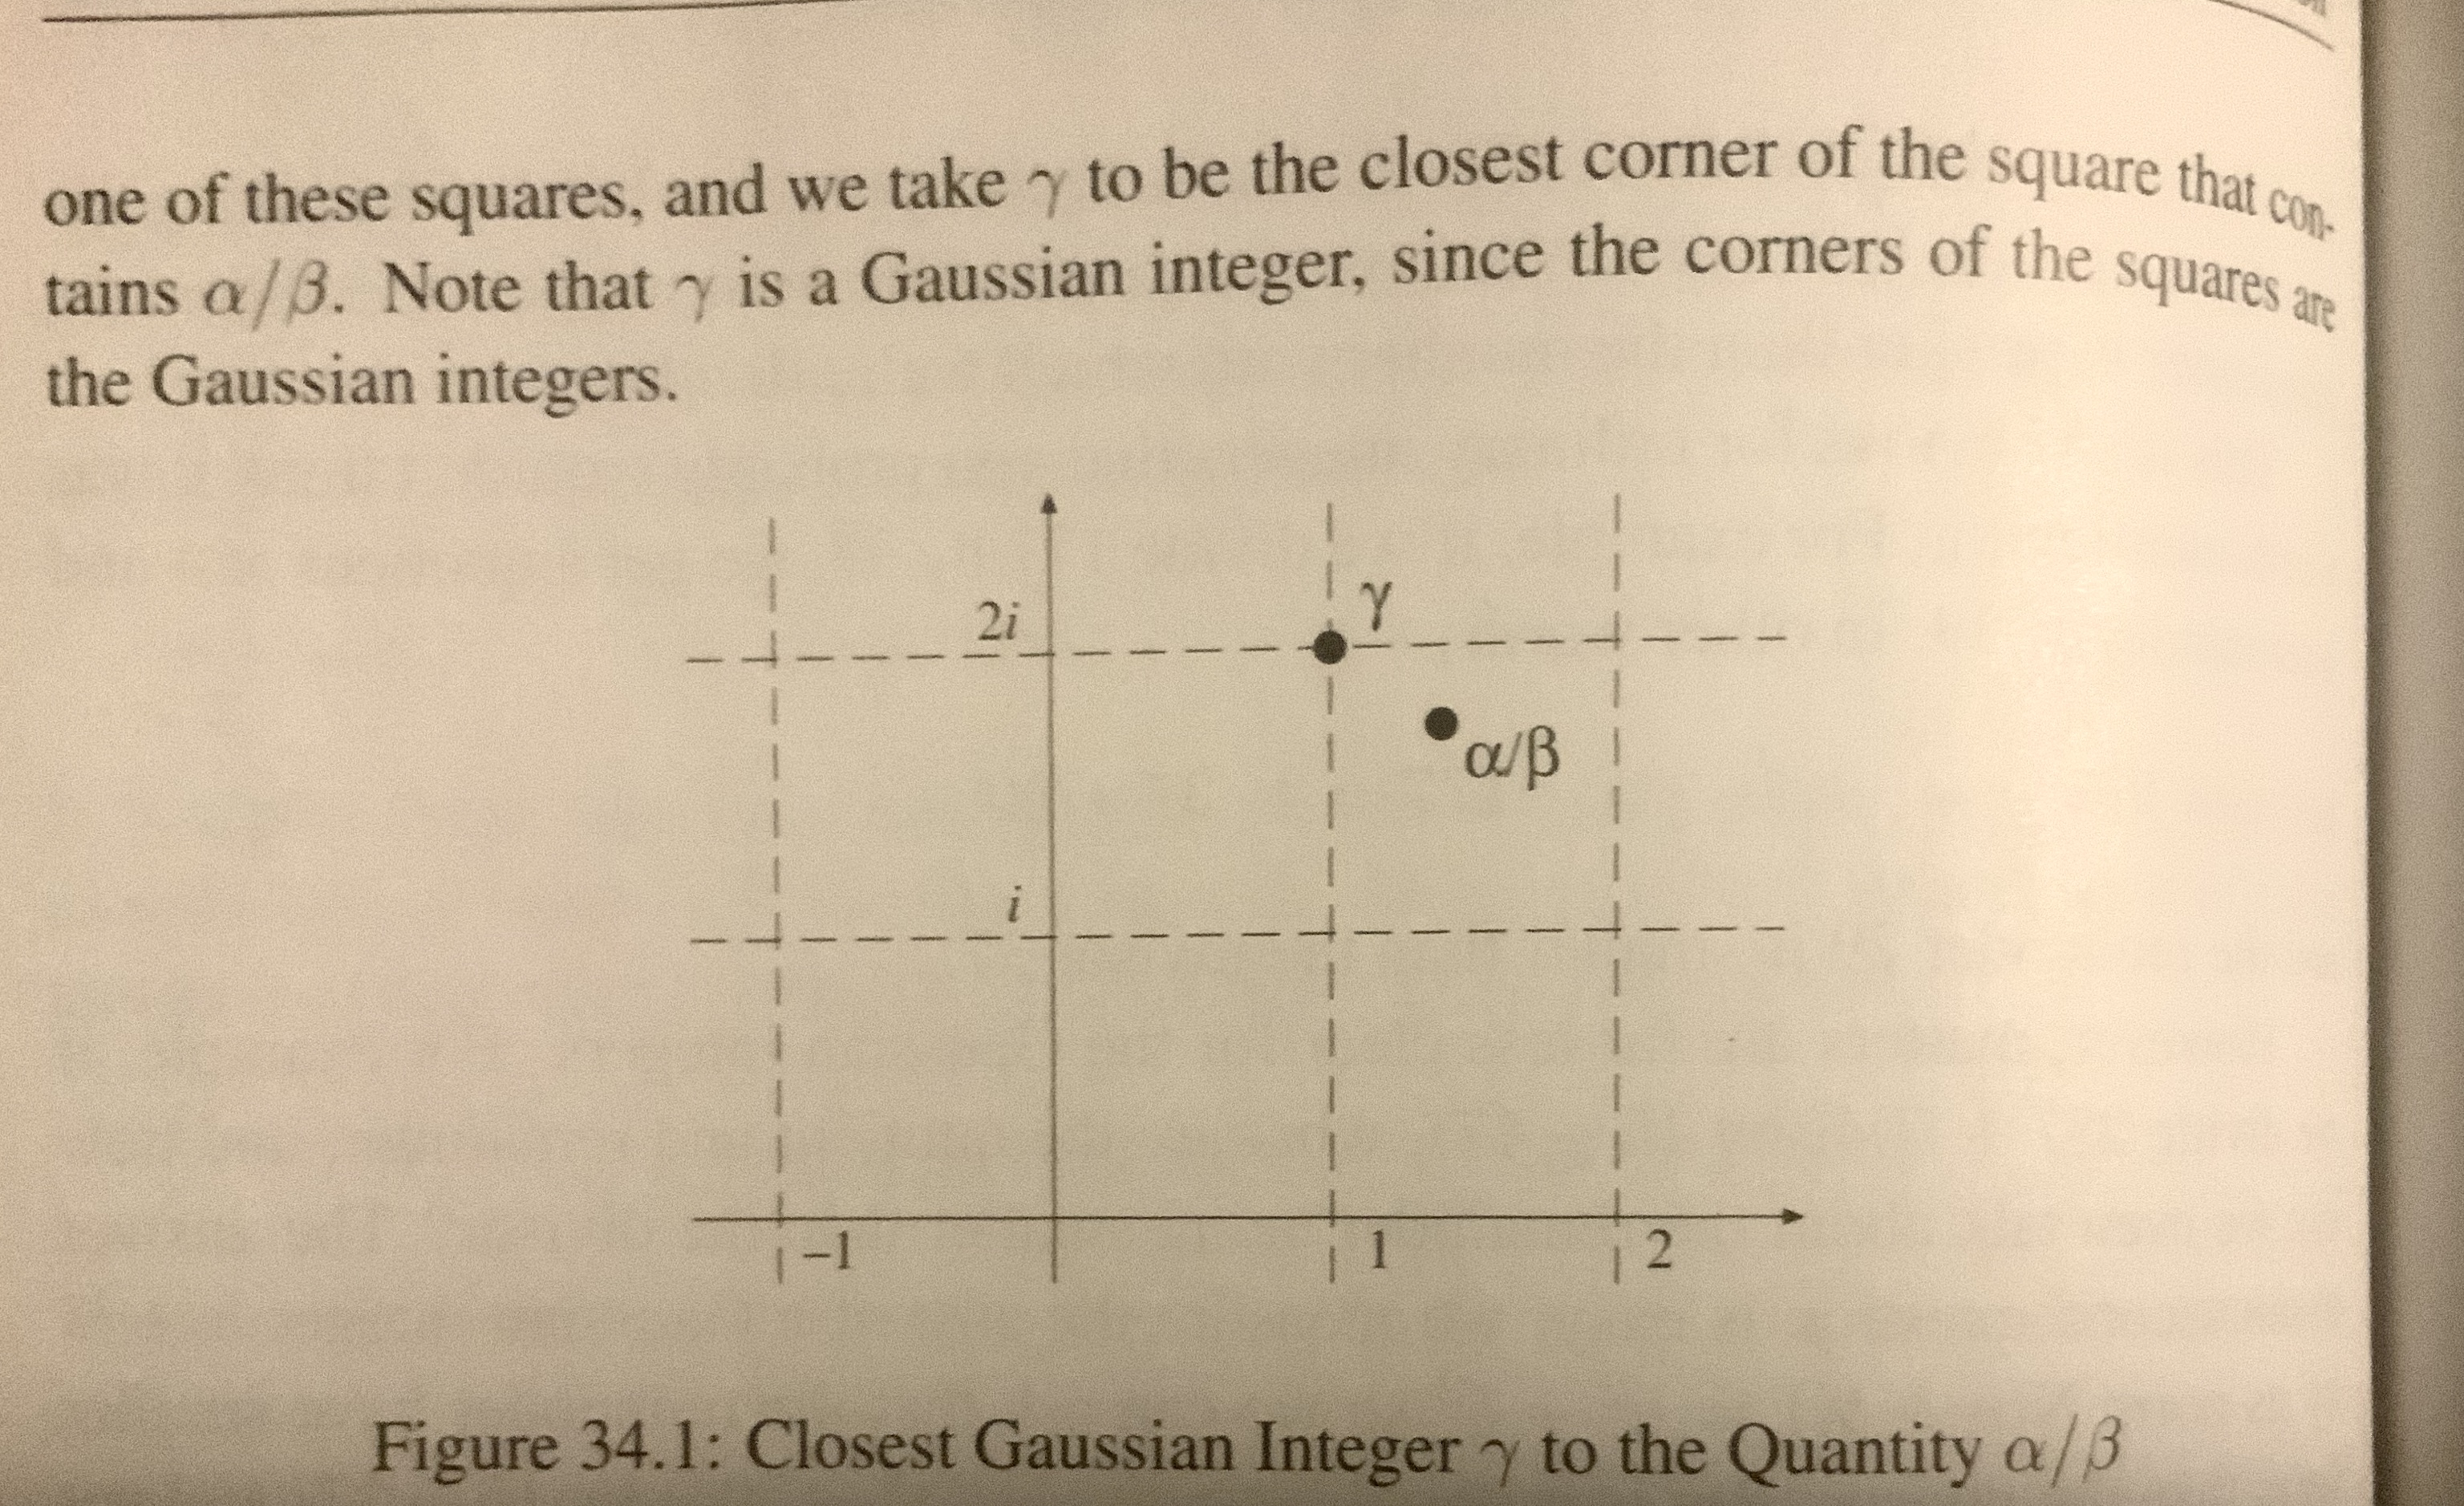
\includegraphics{IMG_0229.jpg}
\end{image}

The farthest that $\frac{\alpha}{\beta}$ can be from $\gamma$ is when it is the middle of the circle $(\textrm{Distance from $\frac{\alpha}{\beta}$ to $\gamma$})\leq\frac{\sqrt{2}}{2}$. Now, the norm is also the square of the distance function, so squaring both sides gives $N(\frac{\alpha}{\beta}-\gamma)\leq \frac{1}{2}$.

Multiplying both sides of the equation by $N(\beta)$, we get $N(\alpha-\beta\gamma)\leq \frac{N(\beta)}{2}.$ Now, set $\rho=\alpha-\beta\gamma$, we get  \[\alpha=\beta\gamma+\rho\quad N(\rho)<N(\beta)\]
(and in fact $N(\rho)\leq \frac{N(\beta)}{2}$).
\end{proof}

\end{document}